\documentclass[conference]{IEEEtran}
\usepackage{epsfig}
\usepackage[cmex10]{amsmath}
\usepackage{url}

\usepackage{multirow}
\usepackage{array}
\usepackage{footnote}

\setlength{\parskip}{0pt}
\setlength{\parsep}{0pt}
\setlength{\headsep}{0pt}
\setlength{\topskip}{0pt}
\setlength{\topmargin}{0pt}
\setlength{\topsep}{0pt}
\setlength{\partopsep}{0pt}
\setlength{\floatsep}{5pt}
\setlength{\textfloatsep}{5pt}
\setlength{\intextsep}{5pt}

\widowpenalty=10000
\clubpenalty=10000

\begin{document}
\title{Addressing the P2P Boostrap Problem for Small Overlay Networks}

\author{
%\IEEEauthorblockN{David Isaac Wolinsky, Pierre St. Juste, P. Oscar Boykin,
%and Renato Figueiredo}
%\IEEEauthorblockA{Advanced Computing Information Systems Lab\\
%University of Florida}
}

\maketitle

\begin{abstract}

Peer-to-Peer (P2P) overlays provide a framework for building distributed
applications consisting of few to many resources with features including
self-configuration, scalability, and resilience to node failures.  Such systems
have been successfully adopted in large-scale Internet services for content
delivery networks, file sharing, and data storage.  The bootstrap problem,
finding an existing peer in the overlay, remains a challenge to enabling these
services for small-scale P2P systems.  In large networks, the solution to the
bootstrap problem has been the use of dedicated services, though creating and
maintaining these systems requires expertise and resources, which constrain
their usefulness and make them unappealing for small-scale systems.
Decentralized, P2P systems can be useful in small-scale systems to address privacy
concerns as well as support for network applications that lack dedicated,
centralized bootstrap servers.

This paper surveys and summarizes requirements that allow peers potentially
constrained by network connectivity to bootstrap small-scale overlays through
the use of existing public overlays.  In order to support bootstrapping a
public overlay must support the following requirements: a method for reflection
in order to obtaining a publicly reachable address, so peers behind network
address translators and firewalls can handle incoming connection requests;
rendezvous for discovering remote peers, when the overlay lacks stable
membership; and communication relaying to share public addresses and
communicate when direct communication is not feasible.  After presenting a
survey of various public overlays, we identify two overlays that match the
requirements:  XMPP overlays, such as Google Talk and Live Journal Talk, and
Brunet, a structured overlay based upon Symphony.  We present qualitative
experiences with prototypes that demonstrate the ability to bootstrap
small-scale private structured overlays from public Brunet or XMPP
infrastructures.

\end{abstract}

\section{Introduction}

While P2P overlays provide a scalable, resilient, and self-configuring platform
for distributed applications, their adoption rate for use across the Internet
has been slow outside of large-scale systems, such as data distribution and
communication.  General use of decentralized, P2P applications targeting homes
and small/medium businesses (SMBs) has been limited in large part due to
difficulty in decentralized discovery of P2P systems --- the bootstrap problem
--- further inhibited by constrained network conditions due to firewalls and
NATs (network address translators).  While these environments could benefit
from P2P, many of these users lack the resources or expertise necessary to
bootstrap private~\footnote{In the context of this paper, private implies that
the overlay's purpose is not for general use. Once established, such overlays
can support privacy in communication; however, overlay security is beyond the
scope of this paper.} P2P overlays particularly when the membership is unsteady
and across wide-area network environments where a significant amount of (or
all) peers may be unable to initiate direct communication with each other due
to firewalls and NATs.

Examples of large-scale P2P systems include Skype, BitTorrent, and Gnutella.
Skype is a voice over P2P system, whereas BitTorrent and Gnutella are used for
file sharing.  The bootstrapping in these systems typically rely on overlay
maintainers using high availability systems for bootstrapping, bundling their
connection information with the application for distribution.  When the
application is started, it uses these high availability servers to connect with
other peers in the system.  Alternatively, some services constantly crawl the
network and place peer lists on dedicated web sites. A new peer wishing to join
the network queries the web site and then attempts to connect to the peers on
that list.

In smaller-scale systems, P2P interests focus on decentralization.  For
example, users may desire to run an application at many distributed sites, but
the application lacks dedicated central servers to provide discovery or
rendezvous service for peers.  In contrast, dedicated, centralized P2P service
providers, such as LogMeIn's Hamachi, a P2P VPN, may collect usage data, which
the users may wish to remain private, or are not free to use.

Many applications of small-scale P2P overlays can be envisioned, including
multiplayer games, especially those that never or no longer have dedicated
online services; private data sharing; and even distributed file systems.
Clearly, a small P2P system could be bootstrapped by one or more users of the
system running on public addresses, distributing addresses out-of-band,
instructing their peers to connect to add that address to their P2P
application, and then initiate bootstrapping; but these types of situations are
an exception and not the norm.  Ultimately, users require an approach that can
make decentralized bootstrapping transparent through minimal and intuititive
interaction with the P2P component.

\begin{figure*}[h!t!]
\centering
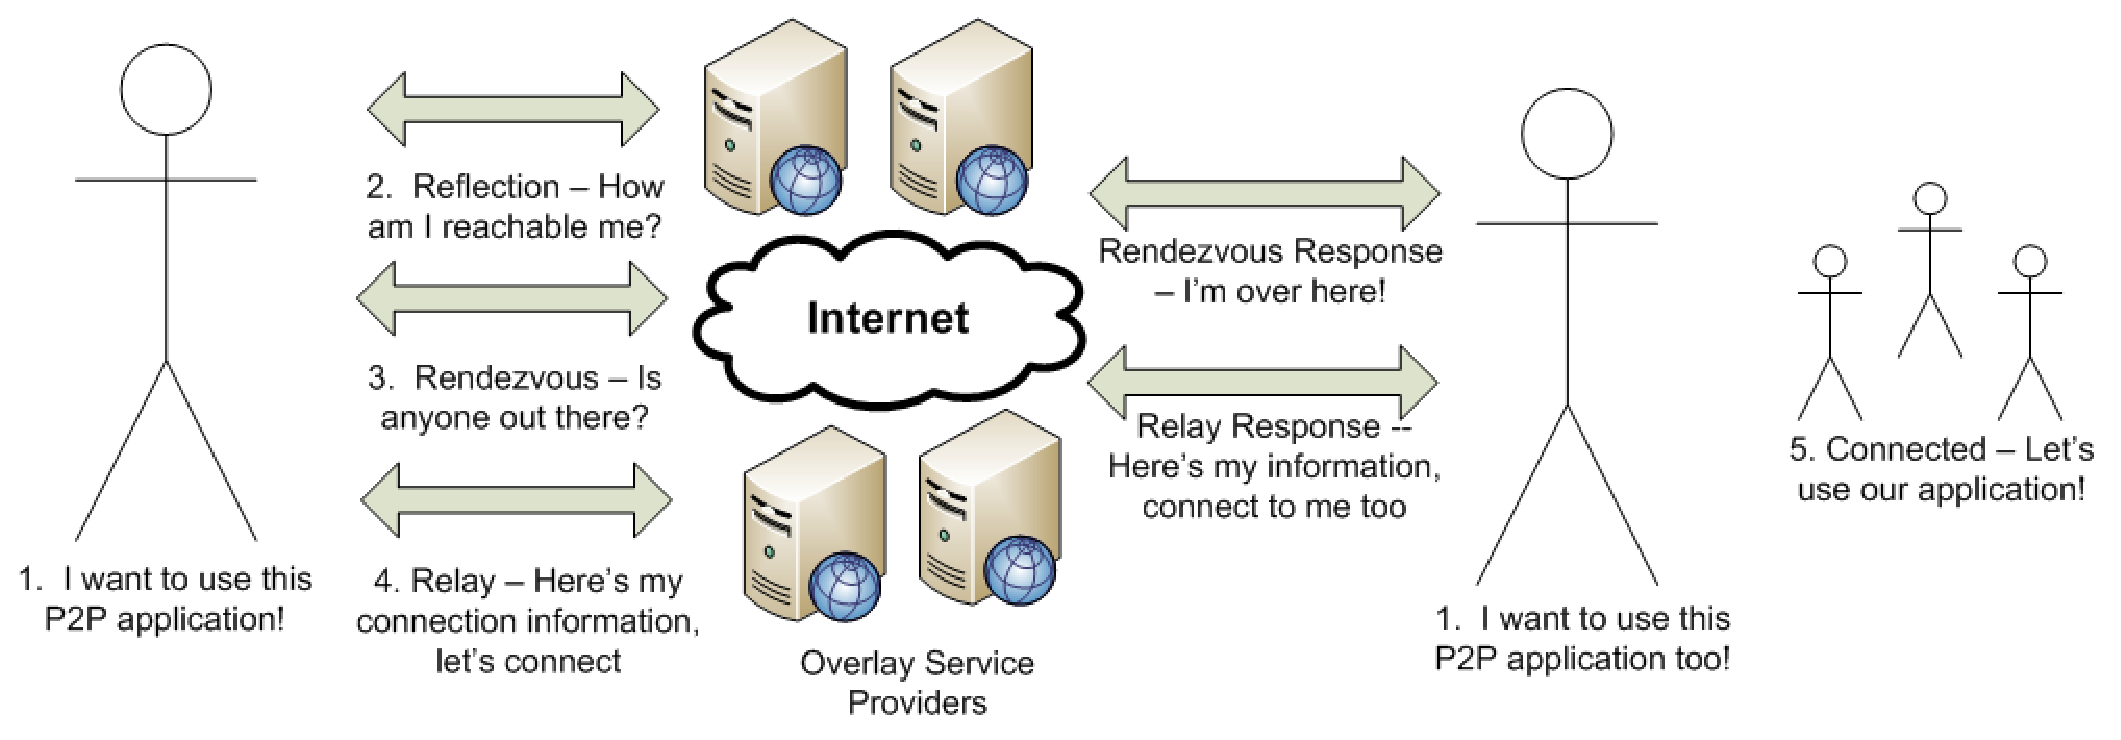
\epsfig{file=figs/bootstrap.eps, width=5.5in}
\caption{Bootstrapping a P2P system using an existing (generic) overlay.}
\label{fig:bootstrap}
\end{figure*}

The basic bootstrapping process can be broken down into two components: finding
a remote peer, and then successively connecting to it and more peers.  When a
node begins, it contacts various bootstrap servers, until it successfully
connects with one, upon which they exchange information.  The bootstrap server
may inquire into the overlay for the best set of peers for the new peer and
respond with that information or it may respond with its existing neighbor set.
At which point, the peer attempts to connect with those peers.  This process
continues aggressively until the peer arrives at a steady state, either
connecting with a specific set of or a number of peers.  Afterwards, the P2P logic
becomes passive, only reacting to churn from new incoming peers or outgoing
peers.

Overlay support for constrained peers, i.e., those behind NATs and restrictive
firewalls, requires additional features to support all-to-all connectivity for
peers in the overlay.  The instantiation of P2P systems for private use could
become overly burdensome, potentially relying on significant human interaction
to bootstrap them, for example, by relaying connection information through
phone calls and e-mail.  Even if this is feasible, this sort of interaction is
undesirable; P2P systems should be self-discovering so that users need to do
minimal amount of work to take advantage of them and ad-hoc systems stress this
point.  In addition, these may rely on centralized components; if they become
unavailable, which is a possibility since most users lack the expertise in
configuring highly available systems, the system will not be accessible.

To address this, we explore the use of existing public overlays as a means to
bootstrap small-scale private overlays.  There are many existing public
overlays with high availability, such as Skype, Gnutella, XMPP, and BitTorrent;
by leveraging these systems, system integrators can easily enable users to
seamlessly bootstrap their own private P2P systems.  In the preceding
paragraphs, we identified the components necessary for bootstrapping a
homogeneous system; now we expand them for environments to support the
bootstrapping of a private overlay from a public overlay with consideration for
network constrained peers.  The public overlay must support the following
mechanisms as illustrated in Figure~\ref{fig:bootstrap}:
\begin{enumerate}
\item \textbf{Reflection} - Constrained peers must have some method of
determining their Internet connection information, to share with other
constrained peers to enable direct connectivity.
\item \textbf{Rendezvous} - Peers seeking members of a private overlay in a
public overlay must be able to identify each other.
\item \textbf{Relaying} - Peers must be able to exchange arbitrary data to
share connection information and to enable direct links across NATs when
possible or, otherwise, as a relay.
\end{enumerate}
This work motivates from the belief that what prevents use of small-scale P2P
systems is due to lack the resources, technical knowledge, and lack of ability
and desire to create and manage high availability bootstrap services.  A public
overlay can be used to transparently bootstrap a private overlay with minimal
user interaction.

The requirements are presented and verified in the context of two prototype
implementations: a XMPP (Jabber)~\cite{xmpp} and Brunet~\cite{brunet}.  XMPP or
Extensible Messaging and Presence Protocol based overlays are commonly used as
chat portals, such as GoogleTalk and Facebook Chat.  XMPP also supports an
overlay amongst servers forming through the XMPP Federation, which allows
inter-domain communication amongst chat peers, so that users from various XMPP
servers can communicate with each other.  Brunet provides generic P2P
abstractions as well as an implementation of the Symphony structured overlay.
We present the architecture for these systems, the lessons learned in
constructing and evaluating them,  as well as provide quantitative analysis of
peer connectivity to a private Brunet overlay.

The organization of this paper follows.  Section~\ref{background} presents
common P2P overlay technologies, motivating examples for this work, existing
solutions to the bootstrapping problem, and NAT challenges in P2P systems.  In
Section~\ref{overview}, we present a survey of overlays, applying the
requirements for private overlay bootstrapping to them, and then show in detail
how they can be applied to Brunet and XMPP.  Our implementation is described in
Section~\ref{implementation}.  In Section~\ref{evaluations}, we then perform a
timing evaluation of bootstrapping overlays using our prototype PlanetLab and
discuss experiences in deploying the system.  Finally, we conclude the paper
with Section~\ref{conclusions}.

\section{Background}
\label{background}

Large-scale P2P systems typically come in two flavors:  unstructured and
structured.  Unstructured systems~\cite{gnutella, fasttrack} are generally
constructed by peers attempting to maintain a certain amount of connections to
other peers in the P2P system, whereas structured systems organize into
well-defined topologies, such as trees, 1-D rings, or hypercubes.  Though
unstructured systems are typically simpler to bootstrap and maintain, they rely
on global knowledge, flooding, or stochastic techniques to search for
information in an overlay, creating potential scalability constraints.
Alternatively, structured systems~\cite{pastry, chord, symphony, kademlia,
can}.  Structured overlays have guaranteed search time typically with a lower
bound of $O(\log N)$ and in some cases even $O(1)$~\cite{beehive}.

Most structured overlays support a decentralized storage / retrieval system
called a distributed hash table (DHT), that maps keys with associated data to
specific node IDs in an overlay.  At a minimum, the data is stored at the node
ID either smaller or larger to the data's key, for fault tolerance the data can
be stored at other nodes.  DHTs can be used by peers of systems to coordinate
allocation and discovery of resources, making them attractive for
self-configuration in decentralized collaborative environments.

Another subset found of P2P systems are those that are not fully decentralized,
such as ``P2P VPNs'' like Hamachi~\cite{hamachi}, older systems like the
original Napster, and tracker-based BitTorrent.  These types of systems provide
a rendezvous services for peers to discover each other to form direct, or P2P,
connections with each other for the purpose of network connectivity or data
sharing.  BitTorrent differentiates itself by using the trackers as a gateway
into the overlay, once inside, peers exchange connection information with each
other directly relegating the tracker as a fall back.  This approach has
enabled BitTorrent to be modified to support trackerless torrents through using
a DHT.

\subsection{Applications}

In this section, we present applications and potential ways to configure them
to use a private overlay.  The work relies on a public key infrastructure and
secure point-to-point and end-to-end communication for P2P as described in our
technical report~\cite{vpo}.  The applications we investigate include chat
rooms, social networks, VPNs, and multicast.  The key to all these applications
is that users can easily host their own services and be discovered through the
use of a free-to-join public overlay.

\subsubsection{Chat Rooms}

Chat rooms provide a platform for individuals with a common interest to find
each other, group discussion, private chat, and data exchange.  One of the most
popular chat systems for the Internet is Internet Relay Chat (IRC).  As
described in~\cite{irc}, IRC supports a distributed tree system, where clients
connect to a server, and servers use a mixture of unicast and multicast to
distribute messages.  The issues with IRC are documented by~\cite{irc_arch},
namely, scalability due to all servers needing global knowledge, reliability
due to connectivity issues between servers, and lack of privacy.  Private
overlays could be extended to support the features of IRC and potentially deal
with these inherent issues.  Each chat room would be mapped to a private
overlay and the public overlay would be used as a directory to learn about
available chat rooms and request access.  Structured overlays could easily be
used as servers for IRC, do not require global knowledge, and can be configured
to handle connectivity issues.

\subsubsection{Social Networks}

Social networks such as Facebook and MySpace provide an opportunity for users
to indirectly share information with friends, family, and peers via a profile
containing personal information, status updates, and pictures.  Most social
network structures rely on hosted systems, where they become the keepers of
user data, which creates privacy and trust concerns.  Private overlays can
remove this third party, making users the only owner of their data.  For this
model, we propose that each user's profile be represented by a private overlay
consisting of their friends.  The overlay should include a secured DHT, where
only all writes are signed to uniquely identify the creator and may only be
removed by the owner of the overlay.  In addition to bootstrapping the private
overlays, the public overlay would be used as a directory for users to find and
befriend each other.  For fault tolerance and scalability, each user provides a
copy of their profile locally, which will be distributed amongst the private
overlay in a read-only DHT, therefore, allowing the user's profile to be
visible whether they are offline or online.  Each user's social network would
than consist of the accumulation of the individual private overlays and the
public overlay.

\subsubsection{P2P VPNs}

Private overlays enable truly decentralized, P2P VPNs.  The most common type of
VPNs are centralized VPNs like OpenVPN, which requires that a centralized set
of resources handle session initialization and communication.  Another approach
taken by Hamachi and many others is to maintain a central server for session
initialization but allow communication to occur directly between peers and
providing a central relay when NAT traversal fails.  SocialVPN~\cite{socialvpn}
relies on a dedicated bootstrap overlay provided by University of Florida.
Using the techniques described in this paper, SocialVPN could be extended so
that it can be bootstrapped into private systems without additional user
configuration.

\subsubsection{Multicast}

The topic of secure multicast has been a focus of much research.  Using an
approach similar to CAN~\cite{can_multicast}, a virtual private overlay forms a
ring where all nodes are members of the multicast group with the additional
feature that you can trust that your audience is limited to those in the
overlay.  The main advantage of such multicasting technologies would be for
wide-area, distributed multicast as described in~\cite{from_peer}.  Examples of
such services include light weight multicast DNS / DNS-SD (service discovery),
as well as audio and video streaming.

\subsection{Bootstrapping P2P Systems}

As described in the introduction, the simple case of bootstrapping is limited
to one peer attempting to find an active peer in the overlay in order for
itself to become a member.  The large-scale providers have resources not
readily available to small-scale overlays.  This section presents the existing
techniques and those being developed and describes their application to
small-scale systems.

When using dedicated bootstraps, a service provider hosts one or more bootstrap
resources.  Peers desiring to join the overlay query bootstrap nodes, until a
successful connection is made to one.  The bootstrap server will then assist in
connecting the peer to other nodes in the P2P system.  Bootstrap nodes are
either packaged with the application at distribution time or through a meta
data file, such as in BitTorrent.  Drawbacks to this approach for small, ad hoc
pools include that the same server would have to be used every time to
bootstrap the system, or users would have to reconfigure their software to
connect to new bootstrap servers over time; at least one peer to have a
publicly accessible address; and it can become a single point of failure.

Another commonly used approach for large-scale systems is the use of a host
cache~\cite{host_cache}.  Clients post current connection information to
dedicated web services, a host cache, that in turn communicate with other host
caches.  For small, ad hoc networks, a host cache acts no differently than a
centralized rendezvous point, requiring that at least one peer has a publicly
accessible address.

``P2P VPN's''~\cite{p2pvpn} use of a BitTorrent tracker is similar to the host
cache concept.  The tracker hosts file meta data and peers involved in sharing.
For the VPN, the peer registers a virtual file that is used to organize the
peers, a form of rendezvous.  When a peer accesses a tracker, it registers its
IP and receives other active ``sharers'' IP addresses.  Peers on public
addresses or using UPNP are able to receive incoming connections from all other
peers.  The problem with this approach is that it is heavily user driven.  A
user must register with each BitTorrent tracker individually and maintain a
connection with each of them, in order to handle cases where BitTorrent
trackers go offline.  In addition, this does not use the BitTorrent trackers in
a normal fashion, so it may be banned by tracker hosts.

Research has shown that peers can use the locality properties of recent IP
addresses in a large-scale P2P system to make intelligent guesses about other
peers in the P2P system using an approach called random
probing~\cite{bootstrapping_p2p, locality_aware}.  The results show for
networks in the order of tens of thousands that a peer can find an active peer
node within as few as 100 attempts and as many as 2,000 guesses.  The
application of this approach to small, ad hoc groups is challenging.  Peers
behind NATs would most likely be unable to receive probe attempts , further
more, if peers are widely distributed and the system small, this approach may
have to query the majority of the IP address range to find a peer.  The results
were not tested in real systems, but instead using overlay traces.

Rather than distribute an IP address, which points explicitly to some location
in the Internet, a small P2P network can apply a name abstraction around one
peer in the overlay using Dynamic DNS~\cite{bootstrapping_ddns}.  In this
approach, peers share a common DNS entry, providing an abstracted mechanism for
labeling the bootstrap peer.  When the peers detect that the IP directed to by
the DNS entry is offline, they replace it with their own.  The application of
this approach to small, ad hoc groups is actually quite nice, as the service
could be distributed across multiple Dynamic DNS registrations.  The
significant drawback to the approach is that the dynamic DNS server could be
attacked, since the login information must be shared amongst all peers in the
overlay.  Also the approach requires that at least one peer be publicly
addressable and know that it is, if a non-publicly addressable peer updates the
cache, it could delay or permanently prevent peers from creating a P2P system.
The results were simulation based and did not determine how well a dynamic DNS
handles rapid changing of name to IP mappings.

IP supports multicasting to groups interested in a common service.  In the case
of bootstrapping a P2P system~\cite{pastry, locality_aware}, all peers would be
members of a specific group.  When a new peer comes online, it queries the
group for connection information and connects to those that respond.  The
approach, by itself, requires that all peers are located in a multicast capable
network, typically spanning only local adrea networks.

A large-scale structured overlay~\cite{one_ring, p2p_bootstrap} could enable
peers to publish their information into a dedicated location for their service
or application and then query that list to obtain a list of online peers.
Peers could search for other peers in their overlay and connect with them using
their connection information.  Since the service would be a large-scale system,
it could easily be bootstrapped by a dedicated bootstrap or host caches.  As it
stands, the described works were position papers and the systems have not been
fully fleshed out.  The primary challenge in relationship to small, ad hoc
networks is that it lacks details bootstrapping of peers behind NATs into
overlays as it provides only a means for rendezvous and no reflection nor
relaying.

\subsection{NAT Hampering the Bootstrap Process}

As of 2010, the majority of the Internet is connected via Internet Protocol
(IP) version 4.  This protocol has a quickly approached limit of addresses
available,  only $2^{32}$ (approximately 4 billion).  With the Earth's
population at over 8 billion and each individual potentially having multiple
devices with Internet connectivity, the IPv4 limitation is becoming more and
more apparent.  Addressing this issue are two approaches:  1) the use of NATs
to enable many machines and devices to share a single IP address but preventing
bidirectional connection initiation, and 2) IPv6 which supports $2^{128}$
addresses.  The use of NATs complicates the bootstrapping of P2P systems as it
prevents peers from simply exchanging addresses with each other to form
connections, as the addresses may not be public.  In addition, firewalls may
prevent peers from receiving incoming connections.  Thus while the eventual
widespread use IPv6 will cause the demise of NATs, though this is not
guaranteed, it does not deal with the issue of firewalls preventing P2P
applications from communicating.

When a machine, \textit{A}, behind a typical NAT, \textit{B}, sends out a
packet to an Internet host, \textit{C}, the NAT device translates the packet so
that it appears it is coming from the NAT device.  The packet sent from
\textit{A} to \textit{C} has the source and destination $IP:port$ pairs
expressed as $IP_A:Port_A$ and $IP_C:Port_C$, respectively.  \textit{A}
forwards the packet to \textit{B} who transforms the source from $IP_A:Port_A$
to $IP_B:Port_B$, where $Port_A$ may or may not be equal to $Port_B$.  This
creates a NAT mapping so that incoming packets from $IP_C:Port_C$ to
$IP_B:Port_B$ are translated and forwarded to $IP_A:Port_A$.

There are a handful of recognized NAT devices as presented in~\cite{stun,
p2p_nats_rfc}.  The following list focuses on the more prevalent types:
\begin{itemize}
\item \textbf{Full cone} - All requests from the same internal IP and port are
mapped to a static external IP and port, thus any external host can communicate
with the internal host once a mapping has been made.
\item \textbf{Restricted cone} - Like a full cone, but it requires that the
internal host has sent a message to the external host before the NAT will pass
the packets.
\item \textbf{Port restricted cone} - Like a restricted cone, but it requires
that the internal host has sent the packet to the external hosts specific port,
before the NAT will pass packets.
\item \textbf{Symmetric} - Each source and destination pair have no relation,
thus only a machine receiving a message from an internal host can send a
message back.
\end{itemize}

Because of the nature of NATs two peers behind them attempting to communicate
with each other will not be able to seamlessly exchange correct addressing
information for each other.  Section~\ref{reflection} describes techniques that
enable peers to exchange routable addresses with each other and
Section~\ref{relay} describes relaying solutions, the alternative when two
peers are unable to communicate directly.

\section{Core Requirements}
\label{overview}

As presented in the preceding sections, a solution to bootstrapping small P2P
overlays must address several challenges, namely reflection, rendezvous, and
relaying.  In this section, we present a generic solution to this problem.  At
the basis of our solution is the use of a publicly available free-to-join
public overlay.  In order to support these features the public overlay must
have mechanisms for peers to obtain a public network identity, reflection;
search for other peers that are bootstrapping the same P2P service, rendezvous;
and send messages to peers through the overlay, relaying.  These are the
minimum requirements to bootstrap a decentralized, P2P system when all peers
are behind NATs.

\subsection{Reflection}
\label{reflection}

Without a reflection, two peers on different networks with non-public addresses
would not have routable addresses with which to communicate with each other.
For constrained resources, the two solutions for traversal are hole punching
and relaying.  In hole punching two peers attempt to form a direct connection
by tricking the NATs to believe that the internal peer has already established
communication with the external peer.  This works, because both peers do it
simultaneously.

In IP communication, the simplest method for NAT traversal is the multiplexing
of a single UDP socket, IP address and port combination.  This behavior can be
supported through either local configuration or remote assistance.  The local
configuration approach relies on the local router supporting either
UPNP~\cite{upnp} or port forwarding / tracking.  In many cases, UPNP is not
enabled by default and in most commercial venues it will rarely be enabled.
Port forwarding / tracking require a more detailed configuration of a router,
outside the comfort range of many individuals and is not uniform across
routers.  A peer using UPNP needs no further services, as UPNP enables a peer
to set and obtain both public IP address and port mappings.  Port forwarding
and tracking mechanisms still require that the user obtains and inputs into the
application their public IP address or use in band assistance described next.

In the remotely assisted scenario, a peer first sends a message to a reflection
provider, perhaps using STUN~\cite{stun_rfc}.  The response from the provider
tells the peer from which IP address and port the message was sent.  In the
case of all cone NATs, this will create a binding so that the peer can then
share that IP address and port with other peers behind NATs.  When the two
peers communicate simultaneously all types of cone NATs can be traversed.  So
long as one peer is behind a cone NAT, NAT traversal using this mechanism is
possible.  The situation becomes complicated when both peers are behind
symmetric NATs or when either one of them have a firewall prevent UDP
communication.  While there exist methods to traversing both symmetric and TCP
only NATs, they are significantly more complicated than the reflection approach
provided by STUN.

Peers behind symmetric NATs cannot easily communicate with each other, since
there is no relation between remote hosts and ports and local ports.  Further
complicating the matter is that there are various types of symmetric NATs,
having behaviors similar to the various cone NAT types.  \cite{ice} describes
methods to traverse these NATs so long as there is a predictable pattern to
port selection.  

Unlike UDP, TCP NAT traversal is complicated by the state associated with TCP.
In many systems, the socket API can be used to enable a peer to both listen for
incoming connections and form outgoing connections using the same local
addressing information.  This is allowed in the TCP specification, but this is
a non-traditional method of employing the sockets API.  According
to~\cite{ice-tcp}, this method works for various types of systems though the
success rate on NATs is quite low, 40\%.  Other mechanisms rely on out of band
communication, \cite{pvc}, or use of complicated predictive
models~\cite{tcp-hole-punching}.

These NAT traversal services only deal with a small portion of the bootstrap
problem, reflection.  That is, peers are able to obtain a public address for
receiving incoming connections.  They provide no means for users to exchange
addresses with each other or perform simultaneous open.  To address this issue
many systems incorporate these NAT traversal libraries and use intermediaries
to exchange addresses.

An example application that uses reflection, rendezvous, and relay services is
is Teredo~\cite{teredo}.  Teredo offers globally identifiable IPv6 addresses to
everyone.  The IPv6 address is constructed in a way to maps to a specific
Teredo gateway, client pair.  When two peers using Teredo attempt to connect
with each other after exchanging their IPv6 addresses out of band, the Teredo
servers exchange the clients IPv4 information obtained using a STUN-like
procedure.  The approach is heavily centralized and if the gateway peer goes
offline or becomes saturated, the peers outgoing and incoming requests may be
ignored.  

\subsection{Relaying}
\label{relay}

In an overlay, there exist two forms of relaying:  one to exchange connection
information and to assist in simultaneous connections and the other would be
similar to the TURN style, arbitrary data router.  Without a relaying mechanism
peers behind some of the various types of cone NATs would be unable to
establish direct connections between each other.  In the other case, there
exists no silver bullet, guaranteed method, for dealing with NAT hole punching.
Relays are the only guaranteed solution for NAT traversal, though it does not
come cheaply.  Relaying requires an entity willing to provide the service and
traffic that can handle the potential delay and bandwidth limitations.  In
general, TURN is not very scalable as it requires a dedicated service provider.
The designers of Teredo found relaying unattractive enough that it was not
included in the Teredo package and thus peers behind severely constrained NATs
are unable to communicate with each other.

A decentralized mechanism for relaying is ideal.  In this case, a peer has an
identifier that is loosely coupled with their network identity and even less to
the overlay provider.  When a remote peers sends a message to the identifier,
the overlay should translate the identifier into network level addresses and
forward it to the destination.  This layer of decoupling could enable a
scalable approach to relaying.  

Relaying must, also, be a somewhat reliable enabling peers to exchange various
sized, arbitrary messages.  In this case, somewhat reliable means that the
service provides at a minimum behavior like UDP, which has been described as an
unreliable protocol.  When a peer sends a message, it should expect the remote
peer should receive it in a reasonable amount of time or not at all.  If the
sending peer does not receive a response within a reasonable amount of time,
follow up requests can be sent until successful or it is deemed the remote
party is no longer online.  

Finally, the service should be asynchronous or event driven.  The previous
requirements would allow peers to relay through a message board or even by
posting messages to a DHT.  The problem with these two approaches is that peers
may very well communicate for long periods of time using these services.  That
means the potential for posting large amounts of data to a service that will
retain it and constantly querying the service to determine if an update is
available.  Both of these are highly undesirable and may be viewed as denial of
service or spam attacks.

\subsection{Rendezvous}

Rendezvous enables peers to have a method for having a predetermined mechanism
to discover each other.  In the simplest case, a peer could randomly probe
other peers on the Internet until it finds a matching peer.  This approach is
unreasonable if overlay is small and even more so if the peers are behind NATs,
as the NATs may very well ignore the requests even if a peer behind the NAT
is actively looking for that overlay as well.

Given an overlay, the most straightforward mechanism for rendezvousing is the
use of a broadcast query to determine if any other peers are using the same
service.  In small enough overlays, this is a perfectly reasonable approach,
Though in large scale systems such as Gnutella, the approach would never work.

There is not one unified method to consolidate rendezvous as doing such would
severely limit its capabilities.  Programming rendezvous using the unique
features of an overlay can enable more efficient forms of rendezvous enabling
peers to increase the likelihood of finding a mutual peer and doing so more
quickly.  For example, in the case of a DHT, peers can use a single DHT key
to store multiple values, all of which would be addresses used to communicate
with peers in the overlay.  Alternatively, in a system like BitTorrent, peers
could use the same tracker and become ``seeds'' to the same virtual file.

\subsection{Overlap}

A single public overlay does not need to provide all the components for
bootstrapping the private overlay.  For example, peers could use the the
Limewire / Gnutella Kademlia DHT, Mojito, as a means to register for
rendezvous.  The peer could leave their globally unique XMPP identity in the
DHT.  Another peer interested in the same service would discover this identity
and then could become friends through XMPP, an automatable process.  Once the
friendship has been formed, they can use XMPP as a means for relaying.

Additionally, a single reflection does not need to be limited to obtain
routable IP addresses.  For example, when a peer communicates through a
relay provided by a service, it needs a global address for peers to direct
messages towards it.  A reflection service in this regards could be the
overlays provision of a resource identifier.

\begin{table*}[h!t!]
\centering
\begin{tabular}[c]{|m{1.5cm}||m{5.5cm}|m{3cm}|m{3cm}|m{3cm}|}
\hline & Description & Reflection & Rendezvous & Relay \\ \hline \hline
BitTorrent &
Default BitTorrent implementations rely on a centralized tracker to provide the
initial bootstrapping.  Peers can establish new connections through information
obtained from established connections.  This relegates the tracker as a means
of monitoring the state of the file distribution.  BitTorrent specifies a
protocol, though each client may support additional features not covered by the
protocol.
&
The current specification does not support NAT traversal, though future
versions may potentially use UDP NAT traversal.  At which point, BitTorrent may
support a reflection service.
&
Peers can register as seeds to the same file hash, thus their IP address will
be stored with the tracker.
&
Peers receive each other's IP addresses from the tracker, there is no inherent
relaying.
\\ \hline
Gnutella &
Gnutella is a large-scale unstructured overlay, consisting of over a million
and, primarily, is used for file sharing.  Gnutella consists of a couple
hundred thousand ultra (super) peers to provide reliability to the overlay.
Gnutella is free-to-join and requires no registration to use.
&
Work in progress.  Peers attempt to connect to a sharers resource, though a
"Push" notification reverses this behavior.  Thus a peer behind a NAT can
share with a peer on a public address.
&
Peers can perform broadcast searches with TTL up to 2, when networks consist of
millions of peers, small overlays will most likely not be able to discover each
other.
&
Not explicitly, could potentially utilize ping messages to exchange messages.
\\ \hline
Skype &
Skype is a large-scale unstructured overlay, consisting of over a million
active peers, and primarily used for voice over P2P communication.  Skype, like
Gnutella, also has super peers, though the owners of Skype provide
authentication and bootstrap servers.  Though Skype is free-to-join, it
requires registration to use.
&
Skype APIs provide no means for reflection.
&
Skype supports applications, or add-ons, which can used to transparently
broadcast queries to a users friend to determine if the peer has the
application installed.  Thus Skype does support rendezvous.
&
Skype applications are allowed to route messages via the Skype overlay, but
because Skype lacks reflection, all communication must traverse the Skype
overlay.
\\ \hline
XMPP &
XMPP consists of a federation of distributed servers.  Peers must register an
account with server, though registration can be done through XMPP APIs without
user interaction.  XMPP is not a traditional P2P system, though it has some P2P
features.  XMPP servers on distinct servers re able to to communicate with each
other.  Links between servers are created based upon client demand.  During link
creation, servers exchange XMPP Federation signed certificates.
&
While not provided by all XMPP servers, there exist extensions for NAT
traversal.  GoogleTalk, for example, provides both STUN and TURN servers.
&
Similar to Skype, XMPP friends can broadcast queries to each other to find
other peers using the same P2P service.  Thus XMPP supports rendezvous.
&
The XMPP specification allows peers to exchange arbitrary out of band
communication with each other.  Most servers support this behavior, even
when sent across the Federation.  Thus XMPP supports relaying.
\\ \hline
Kademlia~\cite{kademlia} &
There exists two popular Kademlia systems, one used by many BitTorrent systems,
Kad, and the other used by Gnutella, called Mojito.  Kademlia implements an
iterative structured overlays, where peers query each other directly when
searching the overlay.  Thus all resources of a Kademlia overlay must be
publicly addressable.
&
Existing implementations of Kademlia does not support mechanims for peers to
determine their network identity.
&
Peers can use the DHT as a rendezvous service, storing their connectivity
information in the DHT at key location:  $hash(SERVICE)$.
&
An iterative structured overlay has no support for relaying messages.
\\ \hline
OpenDHT~\cite{opendht} &
OpenDHT is a recently decommissioned DHT running on PlanetLab.  OpenDHT is
built using Bamboo, a Pastry-like protocol~\cite{pastry}.  Pastry implements
recursive routing, peers route messages through the overlay.
&
Existing implementations of Bamboo and Pastry do not support mechanims for
peers to determine their network identity.  Though this is ongoing work.
&
Peers can use the DHT as a rendezvous service, storing their connectivity
information in the DHT at key location:  $hash(SERVICE)$.
&
Because Pastry uses recursive routing, it can be used as a relay.  Furthermore,
extensions to Pastry have enabled explicit relays called virtual
connections~\cite{epost}.
\\ \hline
Brunet~\cite{brunet} &
Brunet like OpenDHT is a freely available DHT running on PlanetLab, though
still in active development.  Brunet creates a Symphony~\cite{symphony} overlay
using recursive routing.
&
Brunet supports inherent reflection services, when a peer forms a connection
with a remote peer, the peers exchange their view of each other.
&
Peers can use the DHT as a rendezvous service, storing their connectivity
information in the DHT at key location:  $hash(SERVICE)$.
&
Like Pastry, Brunet supports recursive routing and even supports relays called
tunnels~\cite{hpdc08_0}.
\\ \hline
\end{tabular}
\caption{}
\label{tab:overlays}
\end{table*}

\section{Implementations}

Table~\ref{tab:overlays} reviews various overlays, the majority of which are
high availability, public, free-to-join overlays, though some research only
overlays are included.  From this list, we chose to extend Brunet and XMPP to
support private overlay bootstrapping.  Brunet provides a structured P2P
infrastructure, though lacks an active, large-scale deployment outside of
academic institutions due to being rooted in an academic project.  XMPP, on the
other hand, enables connections between friends with routing occurring across a
distributed overlay.

Our implementation makes heavy use of the transports incorporated into
Brunet~\cite{brunet}.  The key distinguishing feature of this library is the
abstraction of sending over a communication link as it supports primitives
similar to ``send'' and ``receive''.  In the next sections, we will describe
how we extended Brunet to be self-bootstrapping as well as extensions to enable
bootstrapping from XMPP.

Our application of structured overlays as the basis private overlays is unique
in that most publications regarding structured overlays focus on their ability
to scale their ability to scale applications have employed them in the order of
10s to 100s of nodes.  For example, Amazon's shopping cart runs on
Dynamo~\cite{dynamo} using a ``couple of hundred of nodes'' or less.  Facebook
provides an inbox search system using Cassandra~\cite{cassandra} running on
``600+ cores''.  Structured overlays simplify organization of an overlay and
provide each member a unique identifier abstracted from the underlying network.
Further more, as mentioned in the cited works, they provide high availability
and autonomic features that can handle churn well.  Further more, when used in
small networks, most structured overlays act as $O(1)$ systems, explicitly
all-to-all though in some cases with relaying, this includes Brunet and Pastry.
Brunet explicitly supports all-to-all though in some cases may require
constrained peers to route through relays.  This can further be ensured by
setting the amount of near connections for the infrastructures, which in Brunet
is configurable at run time.

The XMPP library we used is called Jabber-Net.  Each connection between peers
is uniquely identified by employing socket like concepts, i.e., a pair of
addresses and ports.  The basic representation for this constitutes a pair of
identifiers of the form ``brunet://P2P\_ID:PORT'', where each peer has a unique
ID and port associated for the local and remote entity.  The XMPP
implementation has a similar format: ``xmpp://USERNAME@DOMAIN:PORT/RESOURCE'',
again one identifier for the local peer and one for the remote.

\subsection{Bootstrapping Private Overlays Using Brunet}
\label{brunet_bootstrapping}

Prior to our work, Bruent bootstrapped using a recently online cache of peers
and IP multicast.  We have implemented Brunet to support STUN, such that, with
every connection Brunet makes, peers inform each other of their view of the
remote peers network state, a form of passive \textbf{reflection}.
Furthermore, peers route through the overlay their intentions to connect with
each other through ``ConnectToMe'' messages.  Thus when a peer desires a
connection to another, both peers simultaneously attempt to connect to each
other, dealing with the issue of more restrictive cone NATs and the case when
the peer is behind a non-traversable NAT.  To address the situation where two
peers are behind symmetric NATs or one does not allow UDP, Brunet has been
enhanced to support ``Tunnels''~\cite{hpdc08_0}, where peers route to each
other through their other connections.

In Brunet, we chose to use the DHT for \textbf{rendezvous}, as this provides a
scalable and self-maintaining mechanism for maintaining a bootstrap. All peers
interested in a specific service or private overlay obtain a DHT key based upon
a hashing of the service' or private overlay's name.  Peers can then query this
entry in the DHT to obtain a list of peers in the private overlay.  Note, that
Brunet's DHT implementation supports a single key may have many values.  Since
DHTs are soft state, or lease systems, where data is released after a certain
period of time.  Peers must actively maintain their DHT entry.  The DHT is
a lease or soft state system, where (key, value) pairs are inserted into it
with a time to live, after which, the key is removed from the DHT.  Thus a
peer who is online can actively maintain their DHT entry and when the peer goes
offline, it need not explicitly remove the entry.

For \textbf{relaying}, we further extended Brunet's transport library to
support treating an existing overlay as a medium for point-to-point
communication, we call this a ``Subring'' transport.  Thus in the DHT, peers
store their public overlay address.  When the private overlay transmits data
across the public overlay, it sets the protocol type to match a unique value
for the specific overlay and then sends the packet through the greedy routing
mechanisms on the public overlay to the remote peers public overlay address.
In order to instruct peers to establish ``Subring'' links, they exchange an
identifier that instructs them to do so of the form ``brunet://P2P\_ID:PORT''.

The final challenge faced was the application of Brunet's reflection service
for the private overlay.  There were two directions we could have gone.  The
first would have been to extend Brunet to support STUN in each of the remote
servers and then have a private node query them for their public information.
The problem with this approach is that it would require maintaining additional
state, such as figuring out which of the remote peers are on public addresses
and can provide STUN services.

Instead, we opted to multiplex the socket used for the public overlay as it
already had gone through the process of ``reflection''.  We call the
multiplexing of a single socket for multiple overlay ``Pathing''.  In this
context, the public and private overlays are given a virtual transport layer
that hooks into an underlying transport layer, thus not limited purely to
socket transport layers.  When peers exchange identifiers, instead of
transmitting a simple identifier like ``udp://192.168.1.1:15222'', the
``Pathing'' library extends it to ``udp://192.168.1.1:15222/path'', where each
path will signify a unique overlay.

\subsection{Bootstrapping Private Overlays Using XMPP}
\label{xmpp_bootstrapping}

The key features that make XMPP attractive are the distributed nature of the
federation and the openness of the protocol.  As of December 2009, there are
over 70 active XMPP servers in the XMPP Federation~\cite{xmpp_servers}.  These
include GoogleTalk, Jabber.org, and Live Journal Talk.

In XMPP, each user has a unique identifier of the form ``username@domain''.
Where the domain specifies the client XMPP server and the username explicitly
identifies a single individual.  XMPP supports concurrent instances for each
user by appending a resource identifier to the user ID:
``username@domain/resource''.  A resource identifier can either be provided by
the client or generated by the server.  For users in the same domain, the
server forwards the message from source to destination.  When two users are in
different domains, the sender's server forwards the message to the receiver's
server, who then relays it to the receiver.  Peers are able to send text
messages to each other as well as arbitrary binary messages called ``IQ''.

Peer relationships are maintained by the server.  Peer initiate them through an
in band subscription mechanism based upon ``IQ'', allowing clients to handle
the process of adding and removing peers.  Once peers have established a
connection or subscription, they are informed through a ``Presence''
notification that the peer has come online, this include the full user
identifier.

The \textbf{reflection} component in XMPP is available only to those servers
that support a feature called ``Jingle''~\cite{jingle}.  ``Jingle'' uses ``IQ''
to determine available STUN and TURN servers.  Fortunately, these services are
provided free of charge through GoogleTalk.  In Brunet, we extended the UDP
transport to support querying STUN servers so that it can obtain an address
mapping and keep it open.  STUNs protocol sets the first two bits to 0 in all
messages, thus we used that and the STUN cookie to distinguish it from other
messages.

\textbf{Rendezvous} can be approached in two methods.  We could simply
broadcast a discovery ``IQ'' to all our peers looking for a remote service,
though this may be viewed by the server as some sort of attack.  Alternatively,
a resource identifier could be used to set apart P2P peers from chat peers.
The problem with this approach is what if two P2P applications use the same
base identifier.  Our solution combines the two approaches, so that during the
Presence notification, a peer learns about potential P2P peers.  Then when the
peer is actively querying for remote addresses, it will also inform the queried
peer about the type of P2P service requested.  If the peer's having matching
P2P services, the peer will return a list of addresses otherwise it returns an
empty list.

In order to support the situation, where two peers are unable to communicate
through the exchanged addresses, we have extended XMPP ``IQ'' as a transport to
support \textbf{relaying}.  In the exchanged addresses from the rendezvous phase,
one of the addresses is of the form ``xmpp://username@domain/resource''.  Once
a peer has formed a connection through XMPP, they are then able to attempt
simultaneous connection attempts, further increasing the likelihood of a
connection.  If that does not succeed, the peers can still relay through XMPP.
This approach also has the benefit that, if a XMPP server does not support
``Jingle'', the two peers can still form links with each other.  Since Brunet
supports reflection, eventually, if one of the peers in the system has a
public address, it will automatically assist the other peers into forming
direct links with each other.

\section{Evaluating Overlay Bootstrapping}
\label{evaluations}
In this section, we present a qualitative evaluation of our prototype
bootstrapping a small-scale network and also share some experiences with
deploying overlays.

\subsection{Deployment Experiments}

The purpose of our experiment is to verify that our techniques work and what
overheads should be expected in using Brunet and XMPP to bootstrap an overlay.
The experiments in no means are rigorous as that would become overly focused on
overheads of Brunet and XMPP, instead this paper is primarily interested in
forming small-scale overlays.  The experiment represents 5 peers desiring
all-to-all direct connectivity a feature transparently available to them if
they bootstrap into a private Brunet overlay.

This experiment relied on a public Brunet overlay consisting of over 600 nodes
running on PlanetLab.  PlanetLab~\cite{planetlab} is a consortium of research
institutes sharing hundreds of globally distributed network and computing
resources.  PlanetLab provides a very interesting environment as there is
constant unexpected churn of machines due to the extreme load placed on the
resources and unscheduled system restarts.  Complementary to simulation,
PlanetLab gives us a glimpse of what to expect from the P2P software stack when
used in an actual environment subject to higher variance due to resource
contention and churn.

GoogleTalk provided the XMPP overlay used in this experiment.  Though this
experiment does not take into advantage the features of the XMPP Federation,
this aspect is presented in more detail in the next section reviewing
experiences deploying overlays using XMPP.

\subsection{Deployment Experiences}

In this section, we share some our experiences in deploying XMPP overlays.
Recently, Facebook announced that they would be supporting XMPP as a means to
connect into Facebook chat.  This was rather exciting and further motivated
this work, as Facebook has over 400 million active users, which would have made
there XMPP overlay, potentially, the largest free-to-join overlay.
Unfortunately, experiments established that Facebook does not actually employ a
traditional XMPP setup.  The Facebook XMPP setup merely provides a proxy into
their chat network, preventing features like arbitrary IQs and other forms of
out-of-band messages to be exchanged between peers.  That alone was not the
nail in the coffin, as messages could have still been exchanged encoding the
binary data as text messages between peers.  The nail in the coffin was that
translation performed on peers identifiers.  For example, a user would generate
a XMPP identifier of the form ``username@chat.facebook.com/resource'', but to
its peers, it would be presented as ``uSOME\_NUMBER@chat.facebook.com''.  Thus
peers would then need to use another service just to obtain the identity of the
peer and would have no means to tell what the resource identifier is.  The only
approach to bootstrapping would be to broadcast in-band messages to all peers,
the problem with this is that many peers may actually be using the chat system
for chatting.  These peers would receive spam from an overlay bootstrap, which
they may not be very receptive to.  Finally, Facebook is not a part of the XMPP
Federation, thus peers from GoogleTalk cannot chat with peers from Facebook.
Given that there was no way to exchange arbitrary information and the
rendezvous service was crippled, at this point in time, it appears there is no
way to bootstrap an overlay using Facebook.

During initial tests in verifying the workings of the XMPP code base, we
bootstrapped a  private Brunet overlay on PlanetLab through various XMPP
service providers.  Interestingly, GoogleTalk servers seem to ignore machines
on PlanetLab.  Using another provider, the service appeared to crash after 257
instances of the same account were online.  Unfortunately, the provider had no
contact information available, so we were unable to determine if our test
caused the crash.  There was one server that appeared have no trouble hosting
600 concurrent instances of a single XMPP user, ``jabber.rootbash.com''.  The
nodes were able to rendezvous and relay through \textit{rootbash} and form a
connected P2P system.  The setup did not require reflection, as PlanetLab
resources all have public IP addresses.

Once the system was running on PlanetLab, more tests were performed to
determine the ability to bootstrap across the XMPP Federation.  We formed
friendships, or subscriptions, between users across a few different XMPP
service providers.  In the most evaluated case, a single peer on GoogleTalk and
the PlanetLab system using \textit{rootbash}, the GoogleTalk peer would not
always receive presence notifications for all peers online, though always would
receive some.  When a peer began the relaying mechanism, itr would broadcast to
every peer, it rendezvoused or discovered.  When performing this between
GoogleTalk and \textit{rootbash}, the GoogleTalk peer would not receive a
response.  Though in reducing the broadcast to a random selection of 10 peers,
every 10 seconds until the GoogleTalk peer was connected, the peer received
responses.  The behavior indicates that the XMPP servers may have been
filtering to prevent denial of service attacks.  One last note, when
bootstrapping a peer from GoogleTalk into the \textit{rootbash} system, it
always took 1 minute for the node to become fully connected to the private
overlay.  When the peer used \textit{rootbash}, the peer always connected
within 30 seconds.  It seems as if the communication between XMPP servers was
being delayed for some reason.  The same behavior was not experienced, when
chatting between the two peers.

\section{Conclusion}
\label{conclusions}

In this paper, we have established the requirements for bootstrapping small-scale
P2P overlays, reflection, rendezvous, and relaying.  Reflection is required, so
that peers behind NATs and firewalls can obtain a public address to share with
remote peers.  Rendezvous is a common problem, even for large-scale systems,
peers must have a mechanism to find other peers connecting to are are in the
same overlay.  Finally, without relaying, peers behind NATs would be unable to
exchange with each other their public addresses and perform NAT hole punching.

As we surveyed existing overlays, we found two systems that can easily satisfy
the requirements, XMPP and Brunet.  While Brunet can efficiently provide P2P
services, it is an academic setup, XMPP, on the other hand, is production ready
and distributed across many different providers, each offering
interoperability.  The only issue with using XMPP alone is that peers must
already be friends in order to rendezvous.  For future work, we will
investigate how peers can leverage existing DHT deployments, such as Kad or
Mojito, for rendezvous, form friendships automatically in XMPP, and continue
the bootstrap process using XMPP.  Our implementation successfully deals with
the bootstrapping problem for small-scale overlays using decentralized
technique.

%\section*{Acknowledgment}

\bibliographystyle{IEEEtran}
\bibliography{VirtualPrivateOverlays}
\suppressfloats

\end{document}
